\section{Result}
\subsection{Part 1}

\begin{figure}[H]
    \centering
    \subfloat[Spring]{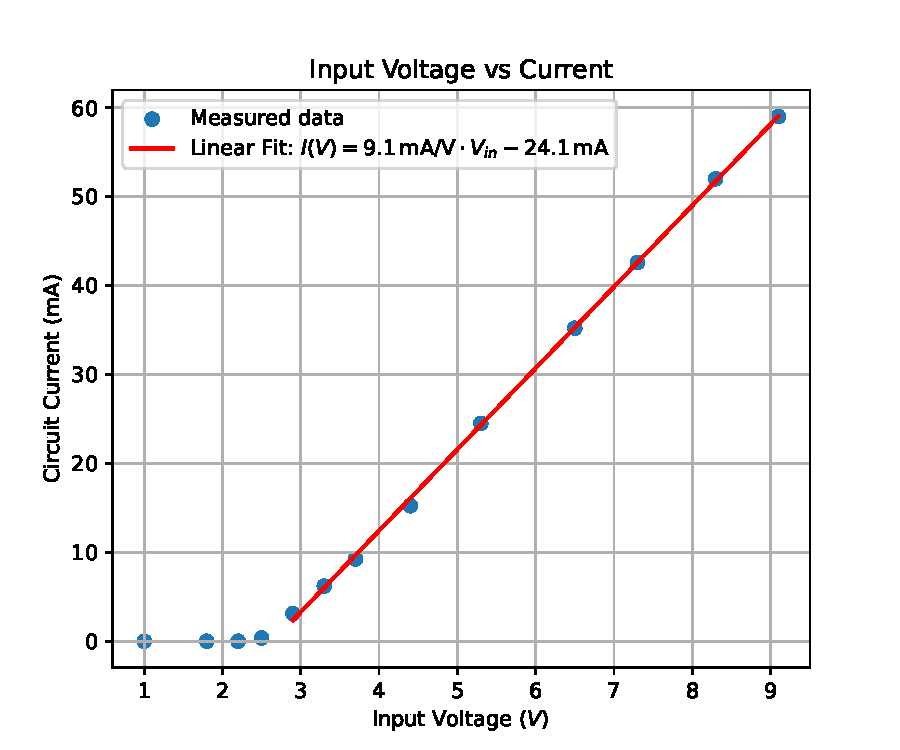
\includegraphics[width=0.49\textwidth]{Figures/part1(a).pdf} \label{fig:a}}
    \hfill
    \subfloat[Summer]{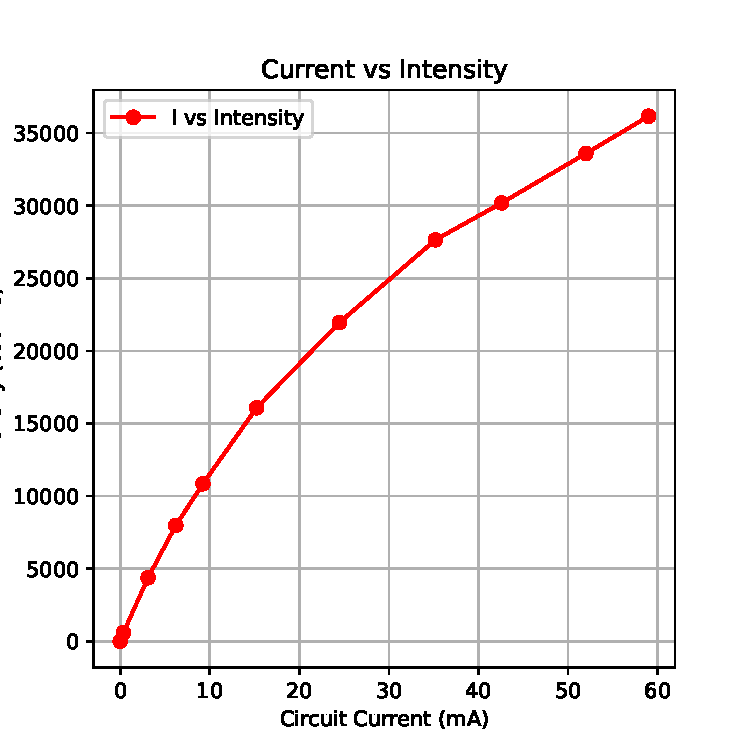
\includegraphics[width=0.49\textwidth]{Figures/part1(b).pdf} \label{fig:b}}
    
    \vspace{0.5cm}
    
    \subfloat[Autumn]{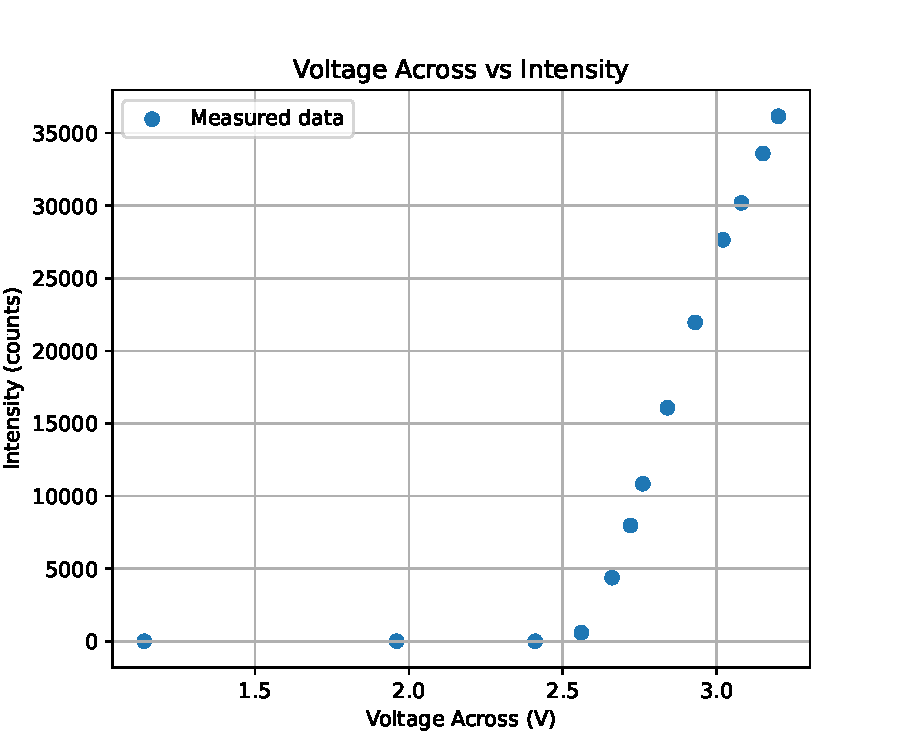
\includegraphics[width=0.49\textwidth]{Figures/part1(c).pdf} \label{fig:c}}

    
    \caption{Histograms for different seasons.}
    \label{fig:part1}
\end{figure}


\subsection{Part 2}

\begin{figure}[H]
    \centering
    \subfloat[Spring]{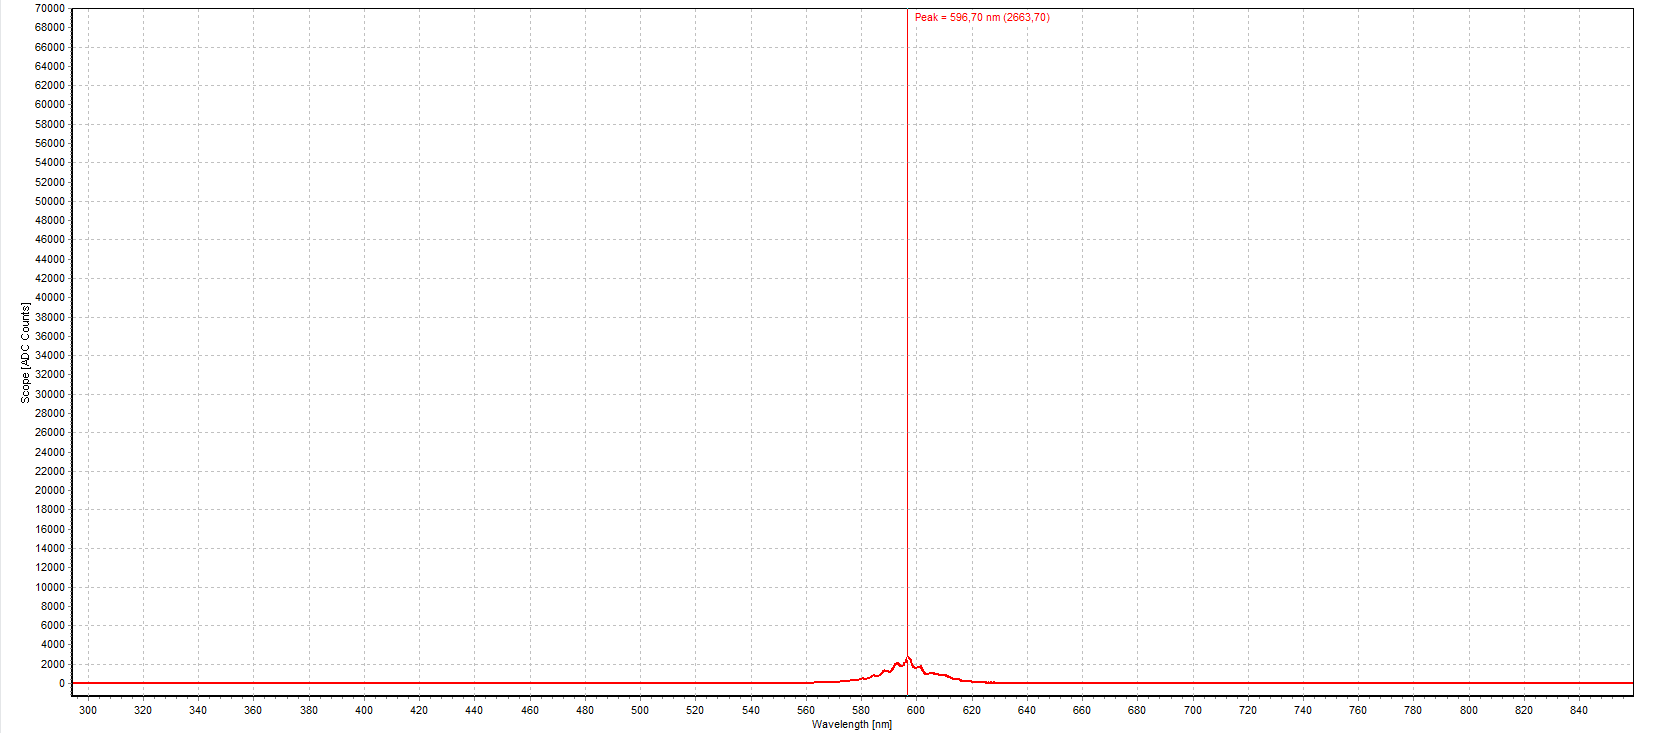
\includegraphics[width=0.9\textwidth]{Figures/Part2_before.png} \label{fig:before}}
    \hfill
    \subfloat[Summer]{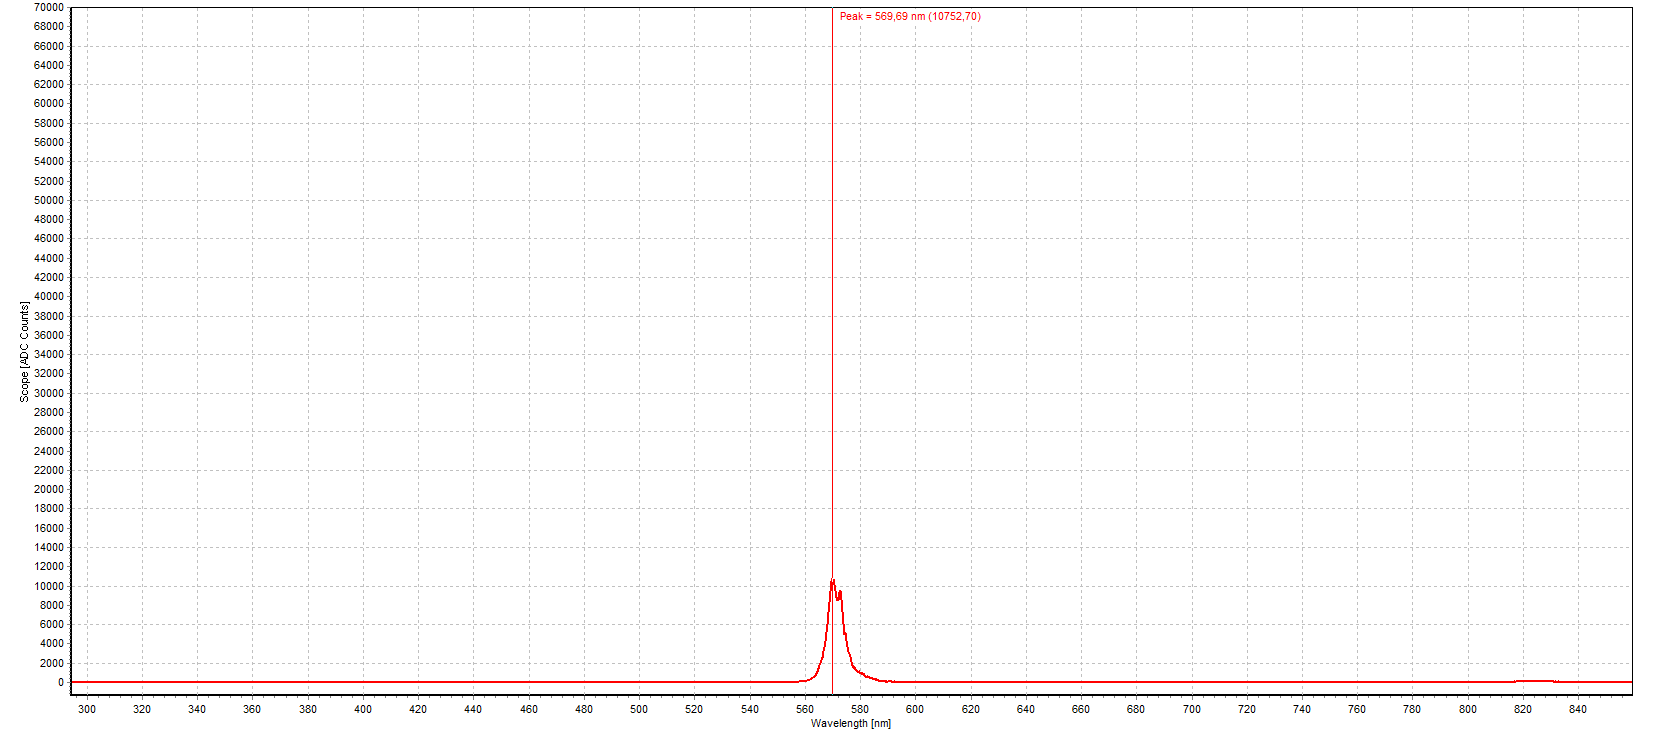
\includegraphics[width=0.9\textwidth]{Figures/Part2_after.png} \label{fig:after}}
    \caption{...}
    \label{fig:part2}
\end{figure}

\subsection{Part 3}

\begin{table}[H]
    \centering
% Please add the following required packages to your document preamble:
% \usepackage{booktabs}
    \begin{tabular}{@{}llll@{}}
    \toprule
    Detector/Emitter & Red    & Green     & Blue      \\ \midrule
    Red              & Output & No output & No output \\
    Green            & Output & Output    & No output \\
    Blue             & Output & Output    & Output    \\ \bottomrule
    \end{tabular}
    \caption{tab:part1}
\end{table}